The proposed algorithm makes use of two concepts to coordinate the voltage regulation between the nodes. They are:
\begin{itemize}
\item Voltage sensitivity analysis
\item Electrical distance calculation
\end{itemize}

\subsection{Voltage Sensitivity Analysis}
The aim of the voltage sensitivity analysis is to determine the effect on the voltage due to reactive power injection at different nodes. Equation (\ref{eq.Pf_equation}) represents the system power-flow equation.  Here ${\Delta Q}, {\Delta P}, {\Delta |V|}$ and ${\Delta \delta}$ represent the change in real power, reactive power, voltage magnitude and voltage angle of nodes. $J$ represents the system jacobian matrix. The elements of $J$ are shown in (\ref{eq.J_equation})
\begin{equation}\label{eq.Pf_equation}
\begin{bmatrix}
{\Delta P}\\ {\Delta Q}
\end{bmatrix} =J\begin{bmatrix}
{\Delta|V|} \\ {\Delta\delta}
\end{bmatrix}
\end{equation}  
Where,
\begin{equation}\label{eq.J_equation}
    J = \begin{bmatrix}
{J_{P|V|}} & {J_{P\delta}}\\ {J_{Q|V|}} & {J_{Q\delta}}
\end{bmatrix}
\end{equation}

Using the components of the system Jacobian matrix the $J_{VQ}$ and $J_{VP}$ matrices can be formulated using (\ref{eq.JVQ}) and (\ref{eq.JVP}).
\begin{equation}\label{eq.JVQ}
    {J_{VQ}} = {J_{Q|V|}}-{J_{Q\delta}}{J_{P\delta}}^{-1}{J_{P|V|}}
\end{equation}

\begin{equation}\label{eq.JVP}
    {J_{VP}}={J_{P|V|}}-{J_{P\delta}}{J_{Q\delta}}^{-1}{J_{Q|V|}}
\end{equation}

Using (\ref{eq.JVQ}) and (\ref{eq.JVP}) the total voltage sensitivity due to real and reactive power injected by a DG can be calculated using (\ref{eq.V_PQ}) \cite{Th_ali}. Here, $[\Delta|V|_{PQ}] , [P_{PV}] $ and $[Q_{PV}]$ represent the total voltage change, real power injected by DG and reactive power injected by DG respectively.

\begin{equation}\label{eq.V_PQ}
[\Delta|V|_{PQ}] ={ J_{VP}}^{-1} [P_{PV}]+{ J_{VQ}}^{-1} [Q_{PV}]
\end{equation}

Using the relation $[P_{PV}] = \frac{[Q_{PV}]}{\cos^{-1}(p.f)}$ equation (\ref{eq.V_PQ}) can be written as
\begin{equation}\label{eq.V_Q}
 [\Delta|V|_{PQ}] ={ J_{VP}}^{-1}\frac{[Q_{PV}]}{\cos^{-1}(p.f)} +{ J_{VQ}}^{-1} [Q_{PV}]
\end{equation}
 Equation (\ref{eq.V_Q}) gives us the relation between total voltage sensitivity and reactive power injection. Here, '$p.f$' represents power factor.

\subsection{Electrical Distance Calculation}
Electrical distance is calculated in order to determine the relative impact on one node due to change in another node. The electrical distances are calculated by determining $M_{sVQ}$ according to equation (\ref{MsQV}) \cite{int1}.

\begin{equation}\label{MsQV}
\begin{bmatrix}
M_{s\alpha}P & M_{s\alpha}Q \\ 
M_{sVP} & M_{sVQ} 
\end{bmatrix} = J^{-1}
\end{equation}
 Here, $J$ is the system jacobian matrix and $M_{s\alpha}P, M_{s\alpha}Q, M_{sVP}$ and $M_{sVQ}$  are the four elements of the inverse of the system jacobian matrix. Equation (\ref{MsVq_expan}) shows the elements of $M_{sVQ}$. \cite{int1}

\begin{equation}\label{MsVq_expan}
M_{sVQ} =
\begin{bmatrix}
\frac{\delta V_{s1}}{\delta Q_{s1}}  & \frac{\delta V_{s1}}{\delta Q_{s2}} & \cdots & \frac{\delta V_{s1}}{\delta Q_{sn}}\\

\frac{\delta V_{s2}}{\delta Q_{s1}}  & \frac{\delta V_{s2}}{\delta Q_{s2}} & \cdots & \frac{\delta V_{s2}}{\delta Q_{sn}}\\

\vdots & \vdots & \vdots & \vdots\\

\frac{\delta V_{sn}}{\delta Q_{s1}}  & \frac{\delta V_{sn}}{\delta Q_{s2}} & \cdots & \frac{\delta V_{sn}}{\delta Q_{sn}}\\ 
\end{bmatrix}
\end{equation}
 
Here $V_{sn}$ and $Q_{sn}$ represent the voltage and reactive power of the node $n$. The electrical distance $D_{sij}$ between the nodes $i$ and $j$ can be calculated using (\ref{ED}) \cite{int1}. 

\begin{equation}\label{ED}
D_{sij} = -\log (\mu_{sij} * \mu_{sji})
\end{equation}

Where,
$$
\mu_{sij} =  \frac{\delta V_{si}}{\delta Q_{sj}} / \frac{\delta V_{sj}}{\delta Q_{sj}}
$$
After determining the electrical distances the nodes are separated into different zones to determine which DG should provide reactive power support for voltage control.

\subsection{Singular value decomposition and pseudo inverse}
In case of a distribution system the system jacobian matrix $J$ is usually a sparse matrix due to the radial nature of distribution systems. Calculating the inverse of $J$ becomes problematic due to this property. For this reason (\ref{eq.V_Q}) and (\ref{ED}) are implemented by determining the pseudo inverse of $J$ using singular value decomposition. The system jacobian matrix $J$ can factored into the expression shown in (\ref{eq.SVD}) \cite{PINV}.
\begin{equation}\label{eq.SVD}
    J = USV^T
\end{equation}

Here, $U$ is an orthogonal matrix whose columns are the eigenvectors of $JJ^T$. $V$ is another orthogonal matrix whose columns are the  eigenvectors of $J^{T}J$. $S$ is a diagonal matrix and is the same size as $J$. Its diagonal elements are the square roots of the nonzero eigenvalues of both $JJ^T$ and $J^{T}J$. The elements of $S$ are the singular values of $J$ and they are represented as $\sigma_1, \sigma_2, ..., \sigma_r$ where $r$ is the rank of $J$. After factoring $J$ into these three components the pseudo inverse of $J$, $J^+$ can be calculated using (\ref{eq.PINV}) \cite{PINV}
\begin{equation}\label{eq.PINV}
    J^+ = US^{+}V^T
\end{equation}
$S^+$ is calculated by taking the reciprocal of all the non-zero elements of $S$ and leaving all the zero elements alone \cite{PINV}.  

\subsection{Control Algorithm}
The core functionality of the algorithm proposed is based on the voltage sensitivity analysis and the concept of electrical distances calculation mentioned before. The main objective of the coordinated voltage control algorithm is the monitoring and control of the voltage at each node of the system, by using inverter-based reactive power and voltage control with traditional voltage regulation devices in order to keep the voltages between the range desired. The calculation of the reactive power needed to be injected is obtained by using the voltage sensitivity and electrical distances concepts. The main steps of the control algorithm is given below.

\begin{enumerate}
%1
\item \textbf{Identify the nodes with voltage limit violation from measured data}
%2
\item \textbf{Determine node with highest voltage deviation.}
%3
\item \textbf{Construct system Jacobian matrix}
%4
\item \textbf{Calculate voltage sensitivity matrix}
%5
\item \textbf{Calculate electrical distances}
%6
\item \textbf{Order the nodes:} In this step, the nodes capable of providing reactive power support are ordered according to their electrical distance from the selected affected node. The ordered list of nodes is saved in a list called \textit{Node\_list}
%7
\item \textbf{Apply the appropriate reactive power:} In this step, the first node in the \textit{Node\_list} is selected. If the node has the capability to supply the required reactive power determined by the sensitivity matrix the algorithm sets the node to provide the required amount of power and continues to \textbf{step 9}. Otherwise, the algorithm sets the node to deliver the maximum available reactive power and takes it out of the list of nodes capable of providing reactive power.
%8
\item \textbf{Repeat steps 3 to 7}
%9
\item \textbf{Estimate new system status:} After deciding the change in node reactive powers the algorithm estimates the new voltage profile of the system using (\ref{eq.Q_V}). If all the nodes in the new estimated profile are within voltage limits the algorithm continues to \textbf{step 10}. Otherwise the algorithm updates the measured data collected from the system with the new estimates and goes back to  \textbf{step 1}.

%10
\item \textbf{Request the devices at the nodes to apply calculated changes}
\end{enumerate}

% \begin{figure}[h]
% \centering
% 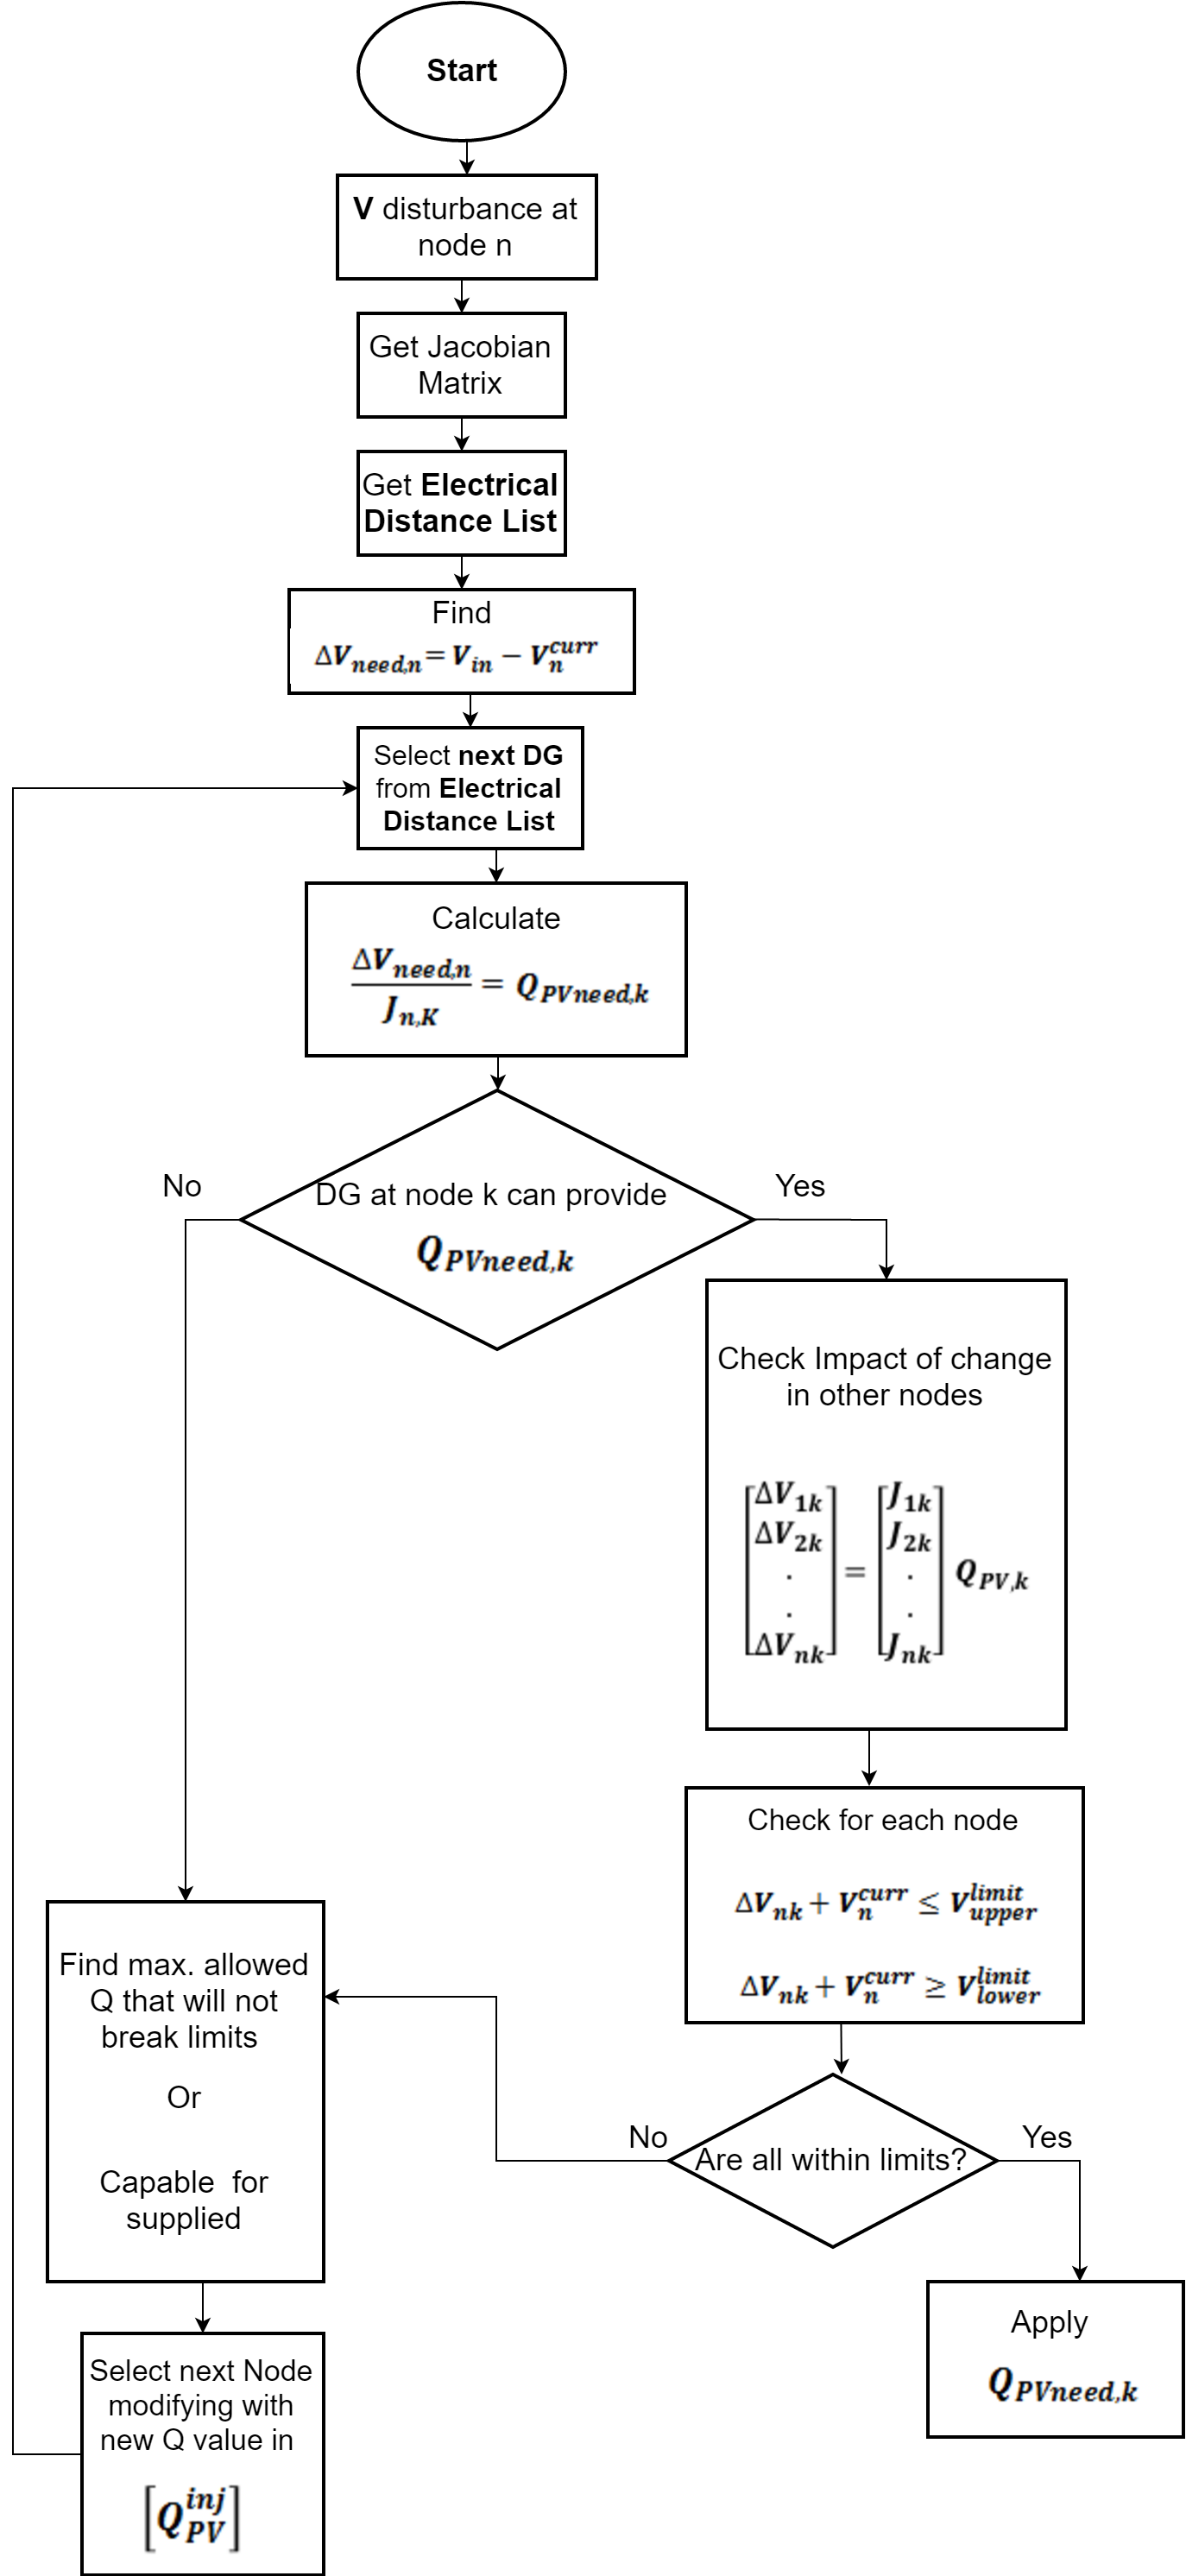
\includegraphics[width=0.5\textwidth]{cvc_alg.png}
% \caption{Coordinated Voltage Control Algorithm Flowchart}
% \label{fig:f1}
% \end{figure}
% The algorithm starts by receiving the needed information from the remote locations. It obtains the voltage and current measurements for each bus and the real and reactive power being generated or absorbed by the DGs. Based on these values, all the voltages are checked against the maximum and minimum voltage range criteria to detect under-voltage or over-voltage issues on specific nodes. When a voltage deviation is detected, the algorithm will start solving the issue from the furthest node to the closest one. The first step in solving this deviation is the application of voltage sensitivity concept to the affected node in order to find the approximate amount of reactive needed be injected at all nodes on control zone of the system. The voltage sensitivity process will return the Jacobian matrix for the system, Jvpq, and the reactive power that each node, in the control zone of the affected bus, needs to individually inject to solve the voltage deviation problem.  After this calculation is completed, a priority list of the nodes on control zone is created based on the criteria of the electrical distances calculated using the method mentioned above. The node closest to the affected node is selected and checked against the nodes that can inject reactive power into the system, in other words, the list of the nodes with DG connected to them. If the node selected to help in the voltage control has the capability of injecting reactive power, the value is checked against all other nodes to assure the compatibility of the value and make sure that no other voltage nodes get out of the desired bounds. As seen on the flowchart, if this value complies with the requirements mentioned, the reactive power reference value is sent to the respective DG inverter. If the value does not comply with the requirements, the next node in the electrical list is selected and the entire process is performed again. Another option for the solution of the reactive power reference calculation, is the application of the maximum reactive power that the current node can supply and the rerun of the entire algorithm to find the solution for the remaining voltage deviation. The algorithm is designed to handle both of these cases and try to minimize the impact in voltage caused by reactive power being injected or absorbed into the system. 




%\subsection{Test System}

